\mySection{11.2 The Method of Least Squares}
%-------------- start slide -------------------------------%{{{ 11.18
\begin{frame}
	% {\S\: 11.2 The Method of Least Squares}
\centering
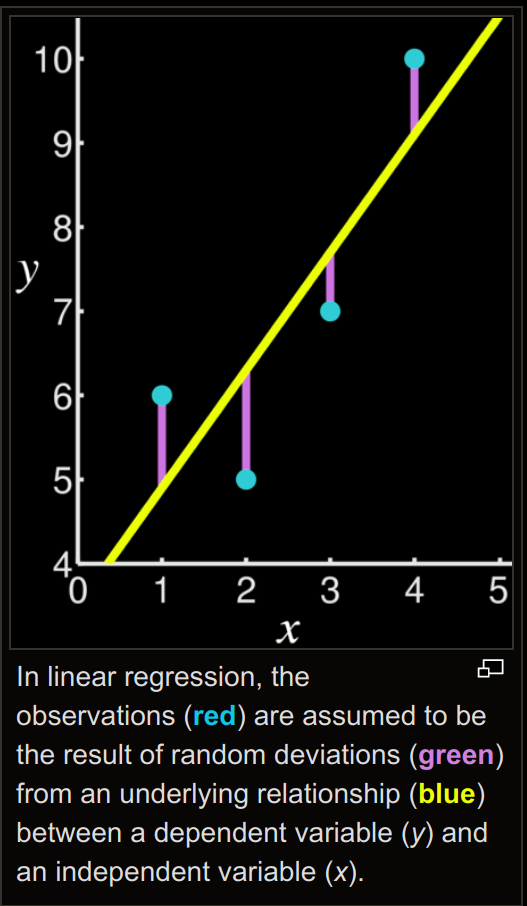
\includegraphics[scale=0.2]{Linear_Regression-neg.png}
\vfill
Goal: Find a blue line that minimizes \\
the sum of the square of the green lines
\end{frame}
%-------------- end slide -------------------------------%}}}
%-------------- start slide -------------------------------%{{{ 11.19
\begin{frame}
\begin{enumerate}
\item[Thm.~] Given $n$ points $(x_1,y_1),\cdots, (x_n,y_n)$, the straight line $y=a+bx$ minimizing \[
		L(a,b) = \sum_{i=1}^n \left[y_i-(a+bx_i) \right]^2
\]
when
\[
b= \frac{n\sum_{i=1}^n x_iy_i - \left(\sum_{i=1}^n x_i\right)\left(\sum_{i=1}^n y_i\right)}{n\left(\sum_{i=1}^n x_i^2\right)-\left(\sum_{i=1}^n x_i\right)^2}
\]
and
\[
a =  \frac{\sum_{i=1}^ny_i-b\sum_{i=1}^nx_i}{n} = \bar y - b \bar x.
\]
\vfill
\item[Proof.]
\begin{align}
\tag{Normal equations}
\begin{cases}
\displaystyle
\frac{\partial }{\partial a}L(a,b) = \sum_{i=1}^n (-2) \left[y_i-(a+bx_i) \right] = 0\\
\displaystyle
\frac{\partial }{\partial b} L(a,b) = \sum_{i=1}^n (-2x_i) \left[y_i-(a+bx_i) \right] = 0\\
\end{cases}
\end{align}
\end{enumerate}
\end{frame}
%-------------- end slide -------------------------------%}}}
%-------------- start slide -------------------------------%{{{ 11.20
\begin{frame}[fragile]
	\[
		\Longleftrightarrow\qquad
\begin{cases}
\displaystyle
\sum_{i=1}^n y_i-n a- b \sum_{i=1}^n x_i = 0& \hspace{5em} (1)\\[1em]
\displaystyle
\sum_{i=1}^n x_iy_i - a \sum_{i=1}^n x_i - b\sum_{i=1}^n x_i^2 =0&\hspace{5em} (2)
\end{cases}
	\]
	\vfill
	\begin{align*}
		(1) & \quad\Longrightarrow \quad a = \bar{y}-b\bar{x}\\[2em]
		(1)\times \sum_{i=1}^n x_i - (2)\times n &\quad\Longrightarrow\quad
	b= \frac{n\sum_{i=1}^n x_iy_i - \left(\sum_{i=1}^n x_i\right)\left(\sum_{i=1}^n y_i\right)}{n\left(\sum_{i=1}^n x_i^2\right)-\left(\sum_{i=1}^n x_i\right)^2}
	\end{align*}
\myEnd
\end{frame}
%-------------- end slide -------------------------------%}}}
%-------------- start slide -------------------------------%{{{ 11.21
\begin{frame}{(Moore-Penrose) Pseudoinverse}

	\begin{enumerate}
		\item Well determined system
			\[
				Ax = b \quad\Longrightarrow\quad x = A^{-1} y.
			\]
			\vfill
		\item Overdetermined system
			\begin{align*}
				Ax &= y\\
				A^T A x &= A^T y \\
				\underbrace{(A^T A)^{-1}A^T A}_{=I} x &= (A^T A)^{-1}A^T y \\
				x &= \underbrace{(A^T A)^{-1}A^T}_{=: A^+} y \\
			\end{align*}
			\vfill
		\item Under determined system
			\[
				Ax= y \quad\Longrightarrow\quad x = \underbrace{A^T(AA^T)^{-1}}_{=:A^+} y.
			\]
	\end{enumerate}
\end{frame}
%-------------- end slide -------------------------------%}}}
%-------------- start slide -------------------------------%{{{ 11.22
\begin{frame}[fragile]

	\begin{enumerate}
		\item[Proof.] (Another proof based on pseudoinverse)
	\[
A =
\begin{pmatrix}
	1 & x_1\cr
	1 & x_2 \cr
	\vdots & \vdots \cr
	1 & x_n
\end{pmatrix}_{n\times 2}, \qquad
x =
\begin{pmatrix}
	\beta_0\cr
	\beta_1
\end{pmatrix}_{2\times 1},\qquad
y =
\begin{pmatrix}
	y_1\cr
	y_2\cr
	\vdots\cr
	y_n\cr
\end{pmatrix}_{1\times n}
	\]
	\vfill
\item[]
	\[
	A^T A =
	\begin{pmatrix}
		1 & 1 & \cdots & 1\cr
		x_1 & x_2 & \cdots & x_n \cr
\end{pmatrix}\begin{pmatrix}
	1 & x_1\cr
	1 & x_2 \cr
	\vdots & \vdots \cr
	1 & x_n
\end{pmatrix}
=
\begin{pmatrix}
	n & \sum_{i=1}^n x_i\cr
	\sum_{i=1}^n x_i & \sum_{i=1}^n x_i^2
\end{pmatrix}
	\]
\vfill
\item[]
\[
	(A^TA)^{-1}  =
% \begin{pmatrix}
	% n & \sum_{i=1}^n x_i\cr
	% \sum_{i=1}^n x_i & \sum_{i=1}^n x_i^2
% \end{pmatrix}^{-1}=
\frac{1}{n\sum_{i=1}^n x_i^2-\left(\sum_{i=1}^n x_i\right)^2}
\begin{pmatrix}
	\sum_{i=1}^n x_i^2
 & -\sum_{i=1}^n x_i\cr
	-\sum_{i=1}^n x_i & n \end{pmatrix}
\]
\end{enumerate}
\end{frame}
%-------------- end slide -------------------------------%}}}
%-------------- start slide -------------------------------%{{{ 11.23
\begin{frame}[fragile]

	\begin{enumerate}
		\item[]
	\[
	A^T y =	\begin{pmatrix}
		1 & 1 & \cdots & 1\cr
		x_1 & x_2 & \cdots & x_n \cr
\end{pmatrix}
\begin{pmatrix}
	y_1\cr
	y_2\cr
	\vdots\cr
	y_n\cr
\end{pmatrix} =
\begin{pmatrix}
	\sum_{i=1}^n y_i \cr
	\sum_{i=1}^n x_iy_i \cr
\end{pmatrix}
	\]
	\vfill
\item[]
	\begin{align*}
		\begin{pmatrix}
			a\cr
			b\cr
		\end{pmatrix}=
x =&
(A^TA)^{-1}A^T y\\[1em]
		=&
\frac{1}{n\sum_{i=1}^n x_i^2-\left(\sum_{i=1}^n x_i\right)^2}
\begin{pmatrix}
	\sum_{i=1}^n x_i^2
 & -\sum_{i=1}^n x_i\cr
	-\sum_{i=1}^n x_i & n
\end{pmatrix}
\begin{pmatrix}
	\sum_{i=1}^n y_i \cr
	\sum_{i=1}^n x_iy_i \cr
\end{pmatrix}\\[3em]
		 =&
		 \begin{pmatrix}
			 \displaystyle
			 \frac{\left(\sum_{i=1}^n x_i^2\right)\left( \sum_{i=1}^n y_i\right) - \left(\sum_{i=1}^n x_i\right)\left(\sum_{i=1}^n x_iy_i\right)}{n\sum_{i=1}^n x_i^2-\left(\sum_{i=1}^n x_i\right)^2} \\[2em]
			 \displaystyle
\frac{n\sum_{i=1}^n x_iy_i - \left(\sum_{i=1}^n x_i\right)\left(\sum_{i=1}^n y_i\right)}{n\sum_{i=1}^n x_i^2-\left(\sum_{i=1}^n x_i\right)^2} \cr
		 \end{pmatrix}
	\end{align*}
	\end{enumerate}
\end{frame}
%-------------- end slide -------------------------------%}}}
%-------------- start slide -------------------------------%{{{ 11.24
\begin{frame}[fragile]
	\[
	b =
\frac{n\sum_{i=1}^n x_iy_i - \left(\sum_{i=1}^n x_i\right)\left(\sum_{i=1}^n y_i\right)}{n\sum_{i=1}^n x_i^2-\left(\sum_{i=1}^n x_i\right)^2}.
	\]
	\vfill
	\begin{align*}
		a=&
			 \frac{\left(\sum_{i=1}^n x_i^2\right)\left( \sum_{i=1}^n y_i\right) - \left(\sum_{i=1}^n x_i\right)\left(\sum_{i=1}^n x_iy_i\right)}{n\sum_{i=1}^n x_i^2-\left(\sum_{i=1}^n x_i\right)^2} \\[2em]
			 =&		 \frac{\left(\sum_{i=1}^n x_i^2\right)\left( \sum_{i=1}^n y_i\right) - \left(\sum_{i=1}^n x_i\right)\left[\left(\sum_{i=1}^n x_iy_i\right)-\frac 1n \left(\sum_{i=1}^n x_i\right)\left(\sum_{i=1}^n y_i\right)\right]}{n\sum_{i=1}^n x_i^2-\left(\sum_{i=1}^n x_i\right)^2} \\[2em]
			 &-  \frac{\frac 1n \left(\sum_{i=1}^n x_i\right)^2\left(\sum_{i=1}^n y_i\right)}{n\sum_{i=1}^n x_i^2-\left(\sum_{i=1}^n x_i\right)^2}\\[2em]
			 =&
			 \frac 1n \sum_{i=1}^n y_i - b\frac{1}{n} \sum_{i=1}^nx_i
			 = \bar{y} -b \bar{x}.
	\end{align*}
	\myEnd
\end{frame}
%-------------- end slide -------------------------------%}}}
%-------------- start slide -------------------------------%{{{ 11.25
\begin{frame}[fragile]{A probabilistic view ... }
\begin{enumerate}
\item[Def.] The function $f(X)$ for which
\[
\E\left[  \left(Y-f(X)\right)^2\right]
\]
is minimized is called the \textcolor{yellow!80!black}{\bf regression curve of $Y$ on $X$}.
\vfill
\item[Thm.] Let $(X,Y)$ be two random variables such that $\Var(X)$ and $\Var(Y)$ both exist.
Then the regression cure of $Y$ on $X$ is given (for all $x$) by
\[
f(x) = \E \left[Y|X=x \right].
\]
\end{enumerate}
\end{frame}
%-------------- end slide -------------------------------%}}}
%-------------- start slide -------------------------------%{{{ 11.26
\begin{frame}
\begin{enumerate}
\item[Proof.] Let $f(x)= \E \left[Y|X=x \right]$ and let $\phi(x)$ be a general function. Then
\begin{align*}
	\E\left[  \left(Y-\phi(X)\right)^2\right]= & \E\left[ \left([Y-f(X)]+ [f(X)-\phi(X)]\right)^2\right]                             \\
	                                         = & \E\left[ \left(Y-f(X)\right)^2\right] +\E\left[  \left(f(X)-\phi(X)\right)^2\right] \\
                                             & +\E\left[ \left(Y-f(X)\right) \left(f(X)-\phi(X)\right)\right].
\end{align*}
\item[] Let $\psi(x)$ be either $f(x)$ or $\phi(x)$. We claim that
\begin{align*}
\E\left[  \left(Y-f(X)\right) \psi(X)\right] =0.
\end{align*}
\item[] Indeed,
\begin{align*}
	\E[Y\psi(X)] & = \iint_{\R^2} f_{X,Y}(x,y)y\psi(x)\ud y\ud x \\
							 & = \int_\R \ud x \psi(x) f_X(x) \underbrace{\int_\R \ud y  \frac{f_{X,Y}(x,y)}{f_X(x)} y}_{\displaystyle = \E[Y|X=x] }\\
							 & = \E[f(X)\psi(X)].
\end{align*}
\item[] Hence,
\[
\E\left[  \left(Y-\phi(X)\right)^2\right]=
\E\left[  \left(Y-f(X)\right)^2\right] +\E\left[  \left(f(X)-\phi(X)\right)^2\right]
\]
which is minimized when $\phi(x)=f(x)$.\myEnd
\end{enumerate}
\end{frame}
%-------------- end slide -------------------------------%}}}
%-------------- start slide -------------------------------%{{{ 11.27
\begin{frame}[fragile]

	\begin{enumerate}
		\item[] If one imposes that $f(x) = a+bx$, then
			\vfill
		\item[Thm.] The following squared error:
			\[
				\E\left[ \left\{ Y - \left( a+b X\right )\right\}^2  \right ]
			\]
		\item[] is minimized at
			\[
				b = \rho_{XY}\frac{\sigma_Y}{\sigma_X}=  \frac{\sigma_{XY}}{\sigma_X^2} \quad
				\text{and}\quad
				a = \E[Y] -b \E[X]
			\]
		\item[] with the mean squared error
			\[
				\E\left[ \left\{ Y - \left( a+b X\right )\right\}^2  \right ] = \left(1-\rho_{XY}^2 \right )\sigma_Y^2.
			\]
	\end{enumerate}
\end{frame}
%-------------- end slide -------------------------------%}}}
%-------------- start slide -------------------------------%{{{ 11.28
\begin{frame}[fragile]

\begin{enumerate}
\item[Proof.]
\begin{align*}
&\E\left[ \left\{ Y - \left( a+b X\right )\right\}^2  \right ]\\
=&
\E\left[ \bigg\{ [Y-\E(Y)] - b[X-\E(X)] - \left[ a-\E[Y] +b \E(X)\right ]\bigg\}^2  \right ]
\end{align*}
\item[]
\begin{minipage}{0.5\textwidth}
	\begin{gather*}
	||\\
\E\left[ \left[Y-\E(Y)\right]^2  \right ]\\
+
b^2 \E\left[ \left[X-\E(X)\right]^2 \right]\\
+ \bigg[ a-\E[Y] +b \E(X)\bigg]^2\\
-2b
\E\bigg[ [Y-\E(Y)] [X-\E(X)] \bigg]\\
-2\bigg[ a-\E[Y] +b \E(X)\bigg] \E\left[ Y-\E(Y)\right]\\
+2b\bigg[ a-\E[Y] +b \E(X)\bigg] \E\left[ X-\E(X)\right]
	\end{gather*}
\end{minipage}
\pause \hfill =\hfill
\begin{minipage}{0.3\textwidth}
	\begin{gather*}
		\Var(Y) \\[0.7em]
		+b^2 \Var(X)\\[0.7em]
		+ \bigg[ a-\E[Y] +b \E(X)\bigg]^2\\[1em]
		-2b\: \Cov(X,Y)\\[1.1em]
		+ 0 \\[1.1em]
+0
	\end{gather*}
\end{minipage}
\end{enumerate}
\end{frame}
%-------------- end slide -------------------------------%}}}
%-------------- start slide -------------------------------%{{{ 11.29
\begin{frame}[fragile]

	\begin{enumerate}
		\item[]
	\begin{gather*}
		\Downarrow\\
\E\left[ \left\{ Y - \left( a+b X\right )\right\}^2  \right ]\\
|| \\
		 \Var(Y)
		+b^2 \Var(X)
		+ \bigg[ a-\E[Y] +b \E(X)\bigg]^2
		-2b\: \Cov(X,Y)
	\end{gather*}
	\vfill
\item[] The best $a$, called $a^*$, should be such that
	\vfill
	\[
		 \bigg[ a^*-\E[Y] +b \E(X)\bigg]^2 = 0
		 \quad\Longleftrightarrow\quad
		 a^* = \E[Y]-b\E[X]
	\]
	\end{enumerate}
\end{frame}
%-------------- end slide -------------------------------%}}}
%-------------- start slide -------------------------------%{{{ 11.30
\begin{frame}[fragile]

\begin{enumerate}
	\item[]
	\begin{gather*}
		\Downarrow\\
\E\left[ \left\{ Y - \left( a^*+b X\right )\right\}^2  \right ]\\
|| \\
		 \Var(Y)
		+b^2 \Var(X)
		-2b\: \Cov(X,Y)\\
		|| \\
		\sigma_Y^2 + b^2 \sigma_X^2 -2b\rho_{XY}\sigma_X\sigma_Y\\
		||\\
		\left(1-\rho_{XY}^2\right)\sigma_Y^2 +
		\bigg(b\sigma_X -\rho_{XY}\sigma_Y \bigg)^2
	\end{gather*}
	\vfill
\item[] The best $b$, called $b^*$, should be
	\vfill
	\[
		\left(b^*\sigma_X -\rho_{XY}\sigma_Y \right)^2 =0
		\quad\Longleftrightarrow\quad
		b^* = \rho_{XY}\frac{\sigma_Y}{\sigma_X}
	\]
\end{enumerate}
\end{frame}
%-------------- end slide -------------------------------%}}}
%-------------- start slide -------------------------------%{{{ 11.31
\begin{frame}[fragile]

	\begin{enumerate}
		\item[]
	\begin{gather*}
		\Downarrow\\
\E\left[ \left\{ Y - \left( a^*+b^* X\right )\right\}^2  \right ]\\
|| \\
\left(1-\rho_{XY}^2\right)\sigma_Y^2
	\end{gather*}
	\vfill
\item[] with
	\vfill
			\[
				b^* = \rho_{XY}\frac{\sigma_Y}{\sigma_X}=  \frac{\sigma_{XY}}{\sigma_X^2} \qquad
				\text{and}\qquad
				a^* = \E[Y] -b \E[X]
			\]
			\myEnd
	\end{enumerate}
\end{frame}
%-------------- end slide -------------------------------%}}}
%-------------- start slide -------------------------------%{{{ 11.32
\begin{frame}[fragile]

\begin{enumerate}
\item[Remark] In practice, we have data $(x_1,y_1),\cdots,(x_n,y_n)$ instead of the joint law of $(X,Y)$ \\
\[\Downarrow\]
\begin{center}
Replace\\[1em]
$\mu_X, \mu_Y, \sigma_X^2,\sigma_Y^2,\rho_{XY}, \sigma_{XY}$
\\[1em]
by their maximum likelihood estimates\\[1em]
$\bar{x},\bar{y},\hat{\sigma}_X^2,\hat{\sigma}_Y^2,r_{XY},\hat{\sigma}_{XY}$
\end{center}
\end{enumerate}
\end{frame}
%-------------- end slide -------------------------------%}}}
%-------------- start slide -------------------------------%{{{ 11.33
\begin{frame}
\begin{enumerate}
\item $\bar x = \frac{1}{n}\sum_{i=1}^n x_i$, $\bar y = \frac{1}{n}\sum_{i=1}^n y_i$\\[2em]
\item $\displaystyle \hat{\sigma}_X^2 =  \frac{1}{n}\sum_{i=1}^n \left(x_i-\bar x \right)^2= \frac{1}{n}\sum_{i=1}^n x_i^2 -\bar x^2=  \frac{n\sum_{i=1}^n x_i^2 - \left(\sum_{i=1}^n x_i \right)^2}{n^2}$
\item[]  $\displaystyle \hat{\sigma}_Y^2 =  \frac{1}{n}\sum_{i=1}^n \left(y_i-\bar y \right)^2= \frac{1}{n}\sum_{i=1}^n y_i^2 -\bar y^2=  \frac{n\sum_{i=1}^n y_i^2 - \left(\sum_{i=1}^n y_i \right)^2}{n^2}$ \\[2em]
\item $\displaystyle \hat{\sigma}_{XY}= \frac{1}{n}\sum_{i=1}^n \left(x_i-\bar x \right)\left(y_i-\bar y \right)=
	\frac{1}{n}\sum_{i=1}^n x_iy_i - \bar{x}\bar{y} $\\[0.5em]
	\hspace{2em}$\displaystyle =  \frac{n\sum_{i=1}^n x_iy_i -
		\left(\sum_{i=1}^n x_i \right)
		\left(\sum_{i=1}^n y_i \right)
	}{n^2}$\\[2em]
\item $\displaystyle r_{XY} =  \frac{\hat{\sigma}_{XY}}{\hat{\sigma}_X \hat{\sigma}_Y}$
\item[]
	\[
	\Downarrow
	\]
	\[
		\boxed{b = r_{XY} \frac{\hat{\sigma}_Y}{\hat{\sigma}_X} = \frac{\hat{\sigma}_{XY}}{\hat{\sigma}_X^2},
		\qquad a = \bar{y}-b\bar{x}}
	\]
\end{enumerate}
\end{frame}
%-------------- end slide -------------------------------%}}}
%-------------- start slide -------------------------------%{{{ 11.34
\begin{frame}[fragile]
	\begin{minipage}{0.45\textwidth}
		\begin{center}
			Maximum likelihood estimates
			\[ \hat{\sigma}_X^2 =  \frac{1}{n}\sum_{i=1}^n \left(x_i-\bar x \right)^2
			\]
			\[
			 \hat{\sigma}_Y^2 =  \frac{1}{n}\sum_{i=1}^n \left(y_i-\bar y \right)^2
			 \]\[
		 \hat{\sigma}_{XY}= \frac{1}{n}\sum_{i=1}^n \left(x_i-\bar x \right)\left(y_i-\bar y \right)
		 \]
		\end{center}
	\end{minipage}
	\hfill
	\begin{minipage}{0.45\textwidth}
		\begin{center}
			Sample (co)variances
			\[ s_X^2 =  \frac{1}{n-1}\sum_{i=1}^n \left(x_i-\bar x \right)^2
			\]
			\[
			 s_Y^2 =  \frac{1}{n-1}\sum_{i=1}^n \left(y_i-\bar y \right)^2
			 \]\[
		 s_{XY}= \frac{1}{n-1}\sum_{i=1}^n \left(x_i-\bar x \right)\left(y_i-\bar y \right)
		 \]
		\end{center}
	\end{minipage}
\end{frame}
%-------------- end slide -------------------------------%}}}
%-------------- start slide -------------------------------%{{{ 11.35
\begin{frame}
\begin{enumerate}
\item[E.g. 1] Producing air conditioners. $x=$ rough weight of a rod. $y=$ finished weight.
Find the best linear approximation of $xy$-relationship.
Predict the weight when $x=2.71$
\\[1em]
\begin{center}
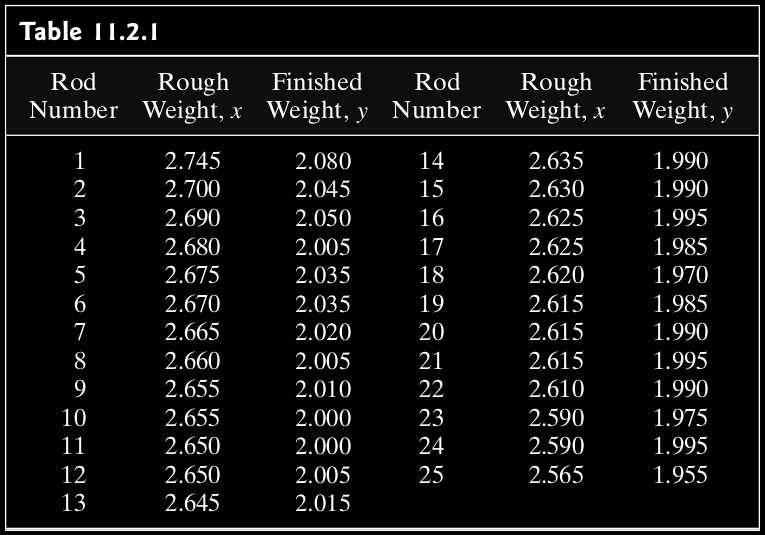
\includegraphics[scale=0.25]{Table_11-2-1-neg.png}
\end{center}
\end{enumerate}
\end{frame}
%-------------- end slide -------------------------------%}}}
%-------------- start slide -------------------------------%{{{ 11.36
\begin{frame}

\begin{enumerate}
\item[Sol.] ...\\[1em]
\vfill
\begin{center}
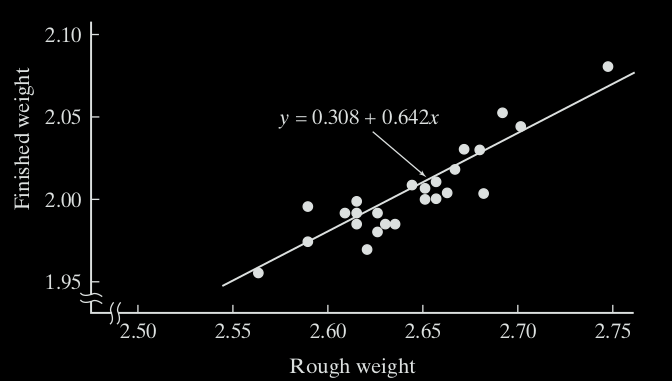
\includegraphics[scale=0.25]{Figure_11-2-1-neg.png}
\end{center}
\vfill
... \myEnd
\end{enumerate}
\end{frame}
%-------------- end slide -------------------------------%}}}
%-------------- start slide -------------------------------%{{{ 11.37
\begin{frame}

\begin{enumerate}
\item[Def.] Let $a$ and $b$ be the least squares coefficients with the sample $(x_1,y_1),\cdots, (x_n,y_n)$.
\\[1em]
\item[] $\hat y=a+bx$: {\bf \textcolor{yellow}{predicted value}} of y
\\[1em]
\item[] $y_i-\hat y_i = y_i - (a+bx_i)$: {\bf \textcolor{yellow}{$i$th residual}}
\vfill
\item[Remark] Use the residual plots to assessing the model.
\end{enumerate}
\end{frame}
%-------------- end slide -------------------------------%}}}
%-------------- start slide -------------------------------%{{{ 11.38
\begin{frame}

\begin{enumerate}
\item[E.g. 1'] Here are the residues and their plots:\\[1em]
\vfill
\begin{minipage}{0.43\textwidth}
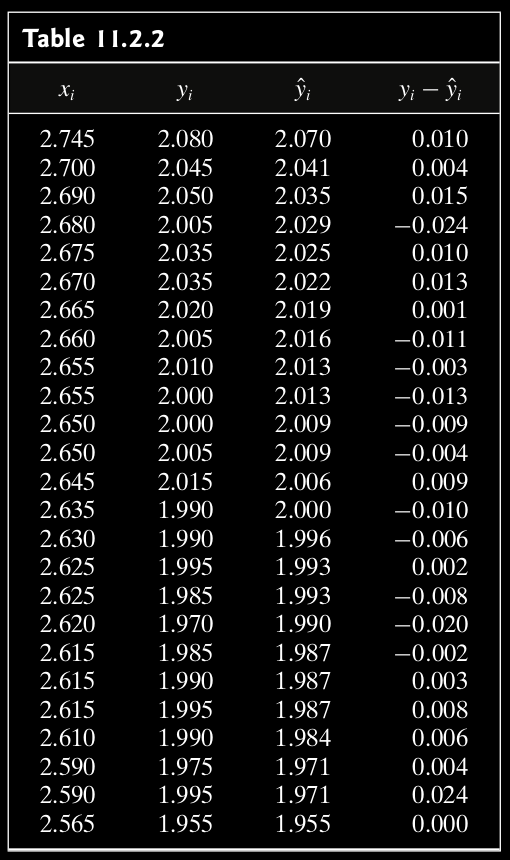
\includegraphics[scale=0.15]{Table_11-2-2-neg.png}
\end{minipage}
\begin{minipage}{0.5\textwidth}
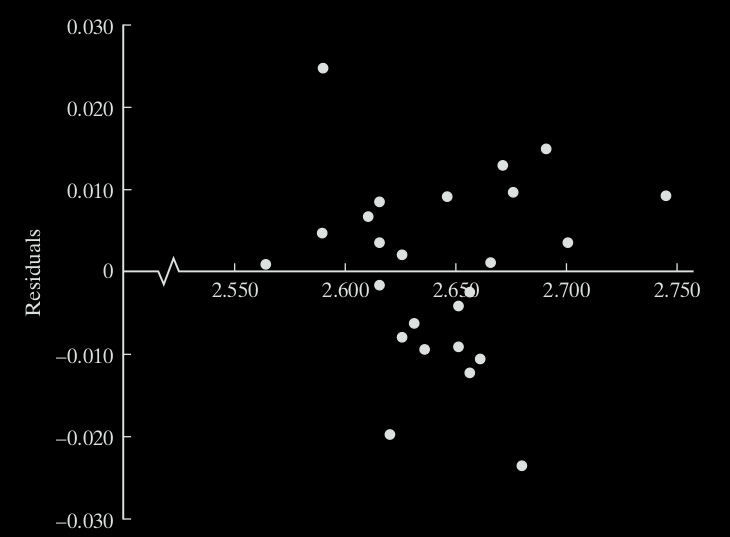
\includegraphics[scale=0.2]{Figure_11-2-2-neg.png}
\end{minipage}
\end{enumerate}

\end{frame}
%-------------- end slide -------------------------------%}}}
%-------------- start slide -------------------------------%{{{ 11.39
\begin{frame}

\begin{enumerate}
\item[E.g. 2] Predict the Social Security expenditures.
\begin{center}
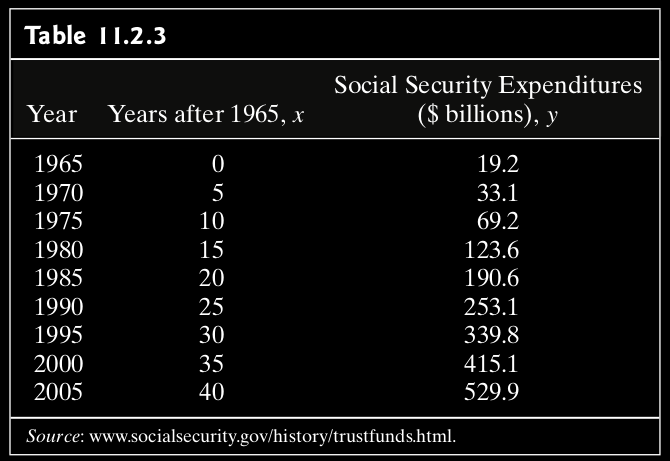
\includegraphics[scale=0.25]{Table_11-2-3-neg.png}
\end{center}
Does the the least squares line $y=-38.0+12.9x$ a good model to predict the cost in 2010 would be $\$543$, i.e., the case $x=45$?
\vfill
\item[Sol.]
\end{enumerate}
\end{frame}
%-------------- end slide -------------------------------%}}}
%-------------- start slide -------------------------------%{{{ 11.40
\begin{frame}
\centering
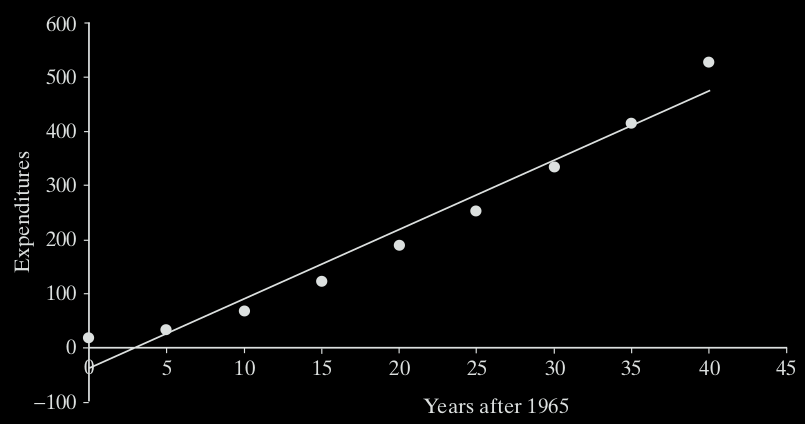
\includegraphics[scale=0.25]{Figure_11-2-3-neg.png}
\\
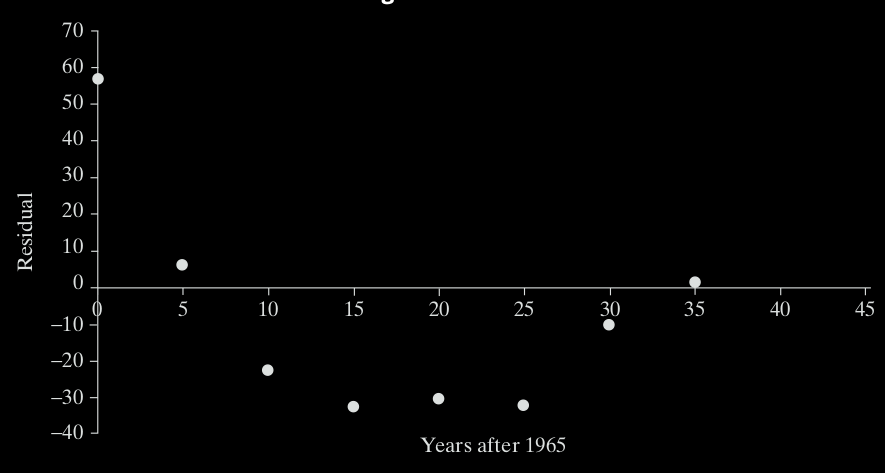
\includegraphics[scale=0.25]{Figure_11-2-4-neg.png}
\end{frame}
%-------------- end slide -------------------------------%}}}
%-------------- start slide -------------------------------%{{{ 11.41
\begin{frame}
	\centering

\includegraphics[scale=0.5]{Nonlinear_regression-neg.png}
\end{frame}
%-------------- end slide -------------------------------%}}}
%-------------- start slide -------------------------------%{{{ 11.42
\begin{frame}{Exponential Regression}
\centering
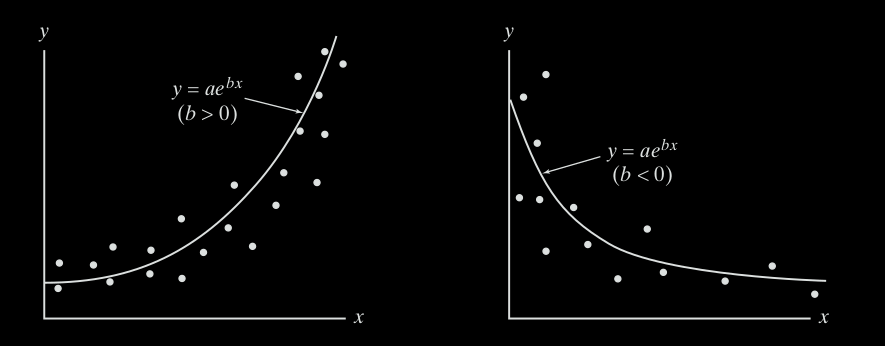
\includegraphics[scale=0.25]{Figure_11-2-7-neg.png}
\vfill
\[
y=a e^{bx} \quad \Longleftrightarrow \quad \ln y = \ln a + b x
\]
\vfill
\[
b= \frac{n\sum_{i=1}^n x_i\alert{\ln y_i} - \left(\sum_{i=1}^n x_i\right)\left(\sum_{i=1}^n \alert{\ln y_i}\right)}{n\left(\sum_{i=1}^n x_i^2\right)-\left(\sum_{i=1}^n x_i\right)^2}
\qquad
\alert{\ln a} =  \frac{\sum_{i=1}^n\alert{\ln y_i}-b\sum_{i=1}^nx_i}{n}
\]
\end{frame}
%-------------- end slide -------------------------------%}}}
%-------------- start slide -------------------------------%{{{ 11.43
\begin{frame}

\begin{enumerate}
\item[E.g.] Moore's law: \\[1em]
Gordon Moore predicted in 1965 that the number of transistors per chip would double every 18 months. \\[1em]
\item[] Based on the real data, check:
\item[] 1) Whether is the chip capacity doubling at a fixed rate?
\item[] 2) Find out the rate.
\vfill
\begin{center}
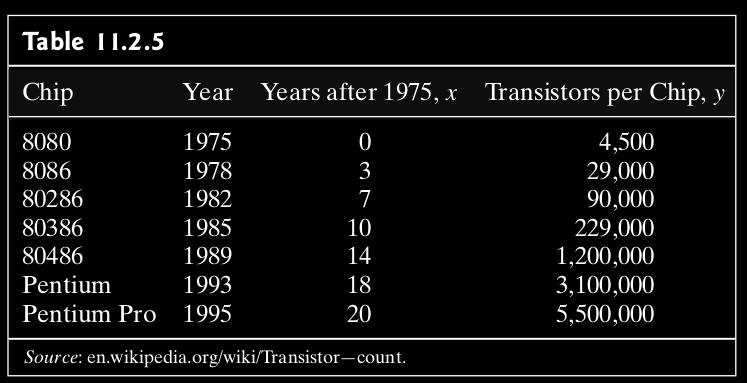
\includegraphics[scale=0.25]{Table_11-2-5-neg.png}
\end{center}
\end{enumerate}
\end{frame}
%-------------- end slide -------------------------------%}}}
%-------------- start slide -------------------------------%{{{ 11.44
\begin{frame}

\begin{enumerate}
\item[Sol.] To check whether chip capacity doubles in a fixed rate, one needs to
carry out exponential regression:
\vfill
\begin{center}
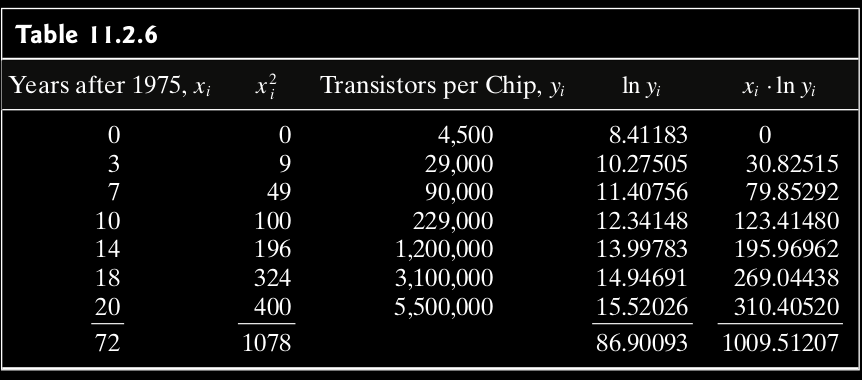
\includegraphics[scale=0.2]{Table_11-2-6-neg.png}
\vfill
\[
\Longrightarrow\quad	b = \cdots = 0.342810, \quad a = \cdots = e^{\ln a} = e^{8.89} = 7247.189.
\]
\vfill
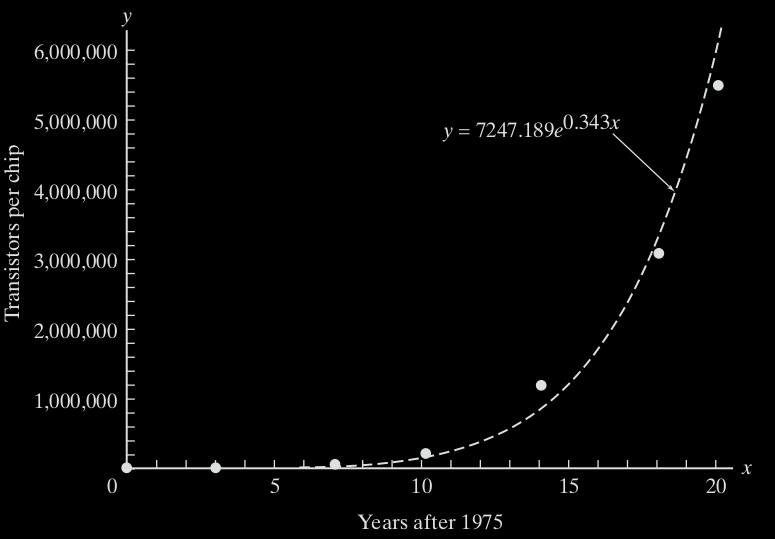
\includegraphics[scale=0.2]{Figure_11-2-8-neg.png}
\end{center}
\end{enumerate}
\end{frame}
%-------------- end slide -------------------------------%}}}
%-------------- start slide -------------------------------%{{{ 11.45
\begin{frame}

\begin{enumerate}
\item[] Finally, to find out the rate:
\vfill
\[
e^{0.343 x} = e^{\ln 2 \times  \frac{0.343}{\ln 2} x} = 2^{ \frac{0.343}{\ln 2}x}
\]
\vfill
\[
\frac{0.343}{\ln 2} x = 1 \quad \Longrightarrow \quad x =  \frac{\ln 2}{0.343} = 2.020837.
\]
\myEnd

\end{enumerate}
\end{frame}
%-------------- end slide -------------------------------%}}}
%-------------- start slide -------------------------------%{{{ 11.46
\begin{frame}{Other curvilinear models}
\centering
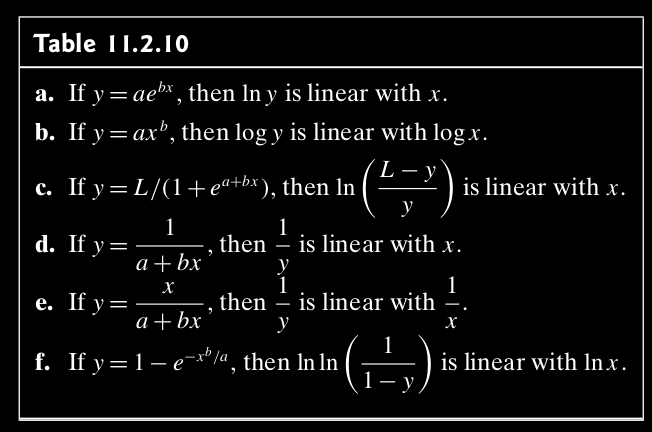
\includegraphics[scale=0.3]{Table_11-2-10-neg.png}
\end{frame}
%-------------- end slide -------------------------------%}}}
